\section{Theoretical Framework: The TPACK Model}

To understand the ``pedagogical'' positioning of Origin AI, we refer to the \textbf{Technological Pedagogical Content Knowledge (TPACK)} framework. Introduced by Mishra and Koehler (2006) \cite{mishra2006technological}, TPACK identifies the nature of knowledge required by teachers (and by extension, intelligent tutoring systems) for technology integration in their teaching, while addressing the complex, multifaceted and situated nature of teacher knowledge.

\begin{figure}[ht]
    \centering
    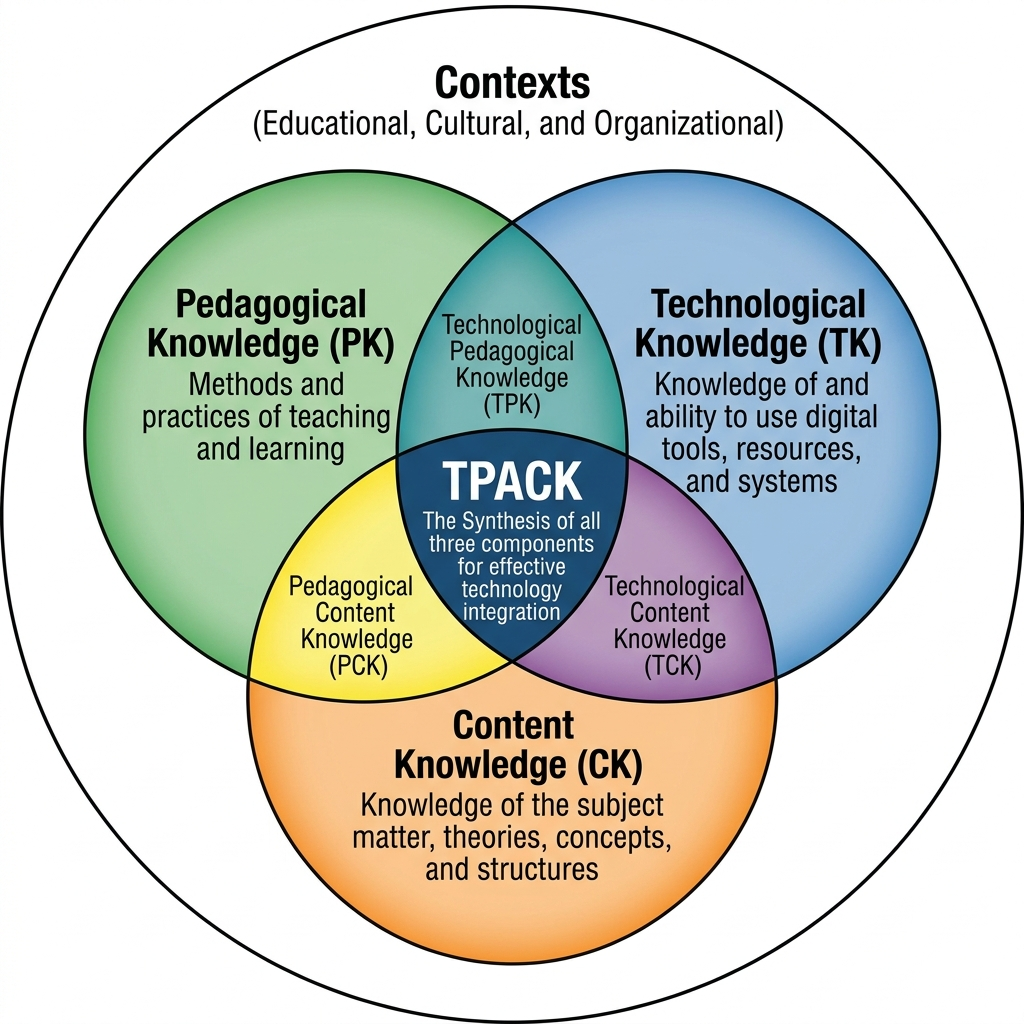
\includegraphics[width=0.6\textwidth]{report_file/tpack_model.png}
    \caption{The TPACK Framework (Source: \cite{tpack_review_2021})}
    \label{fig:tpack}
\end{figure}

The TPACK framework (Figure \ref{fig:tpack}) consists of three main components: Content Knowledge (CK), Pedagogical Knowledge (PK), and Technological Knowledge (TK). The intersection of these three bodies of knowledge forms the basis of effective teaching with technology. Origin AI specifically targets the \textbf{Technological Pedagogical Content Knowledge (TPACK)} intersection by:
\begin{itemize}
    \item \textbf{Content Knowledge (CK):} Utilizing subject-specific knowledge bases (Biology, Chemistry, Physics, Mathematics).
    \item \textbf{Pedagogical Knowledge (PK):} Enforcing hint-first policies and Socratic coaching through AI guardrails.
    \item \textbf{Technological Knowledge (TK):} Leveraging Large Language Models and tiered orchestration for scalable delivery.
\end{itemize}

\section{Traditional RAG Systems and Their Limitations}

Retrieval-Augmented Generation (RAG) systems, introduced by Lewis et al. (2020), have become the standard for grounding LLM responses in external knowledge. A typical RAG pipeline embeds a user query, retrieves relevant document chunks from a vector database (e.g., using cosine similarity), and then feeds those chunks as context to an LLM for answer generation.

While RAG improves factual accuracy and reduces hallucinations compared to bare LLMs, it has several limitations in the educational context. First, every query incurs both embedding and LLM generation costs – typically 1,000+ tokens per query – making it still expensive at scale. Second, retrieval is based purely on semantic similarity, not on pedagogical structure or student context. A retrieved document chunk might contain the correct answer but at the wrong level of detail or with an inappropriate teaching style. Third, there is no prioritization of known answers. If the same question is asked by thousands of students, RAG will retrieve and generate a new answer each time, wasting tokens.

Origin AI improves upon RAG by adding two zero-cost layers before retrieval: stored solution lookup (exact match for common questions) and subject knowledge base lookup (structured pedagogical atoms). Only when both fail does the system fall back to retrieval and then to generation.

\section{Rule-Based Pedagogical Agents}

Early intelligent tutoring systems (ITS), such as Cognitive Tutors developed at Carnegie Mellon University, used rule-based engines to provide step-by-step guidance. These systems encode expert knowledge as production rules (if-then statements) and use them to diagnose student errors and provide feedback.

Rule-based systems are highly predictable, inexpensive to run (no API costs), and can be designed to adhere strictly to curriculum standards. However, they require extensive manual authoring of rules and content, which does not scale well to large, open-ended domains. They also lack the flexibility to handle novel or off-topic student questions. In contrast, Origin AI uses a hybrid approach: local rule-based lookup for known concepts (via the subject KB) and generative LLM fallback for novel queries, combining the predictability of rules with the flexibility of LLMs.

\section{Generic LLM Chatbots in Education}

ChatGPT, Claude, and Gemini have been widely adopted in educational settings, both formally (through institutional licenses) and informally (students using personal accounts). Studies have shown that these tools can be effective for explanation, summarization, and brainstorming.

However, researchers have identified several challenges. First, students often need to provide extensive context (``I'm looking at question 5 on page 32 of the HC Verma textbook...'') before receiving useful help, leading to frustration and abandonment. Second, these models have no concept of test integrity – they will answer any question, even during exams, unless explicitly instructed via system prompts (which can be bypassed by clever prompting). Third, they are not optimized for the specific vocabulary, problem-solving patterns, and marking schemes of competitive exams like JEE and NEET. Finally, the cost of using these models at scale is prohibitive for most educational institutions.

Origin AI addresses each of these issues through its 4-layer context assembly (eliminating manual context description), guardrails (enforcing test integrity), subject-specific knowledge bases (grounding in exam patterns), and tiered pipeline (reducing cost).

\section{Context-Aware Systems and In-Situ Assistance}

The concept of ``context-aware computing'' dates back to the 1990s, with early work on location-aware and situation-aware systems. In the educational domain, context-aware systems have been explored for adaptive learning, where the system adjusts content based on the student's location, time of day, or prior performance.

However, most existing systems focus on coarse-grained context (e.g., ``student is at home'' or ``student has completed 50\% of the course''). Fine-grained, real-time context such as the exact question on the screen, the selected text, and the test status is rarely captured and utilized. Origin AI's PageContext and HighlightContext layers represent a novel application of fine-grained context to AI mentorship, enabling in-situ assistance that feels like a human tutor looking over the student's shoulder.

\section{The Rise of Multimodal Learning Environments}

The integration of multiple sensory channels—text, audio, and visual—in learning environments is grounded in the \textbf{Cognitive Theory of Multimedia Learning (CTML)}, proposed by Richard Mayer. CTML suggests that people learn more deeply from words and pictures than from words alone. In the context of AI mentors, this translates to the ability of the system to process visual context (the question on screen) and provide auditory feedback (voice explanation).

Recent advancements in vision-language models (VLMs) have enabled AI to understand images and UI states with high precision. Origin AI's HighlightContext and PageContext layers are implementations of this trend, allowing the system to bridge the gap between static text and dynamic visual interaction. Research shows that such "in-situ" assistance reduces the cognitive load required for context-switching, thereby improving "Time on Task" for students.

\section{Speech-to-Text (STT) and Text-to-Speech (TTS) in Pedagogy}

Voice interaction is a powerful tool for accessibility and engagement. For students with learning disabilities like dyslexia, or those who simply prefer verbal communication, voice-enabled AI mentors provide a more inclusive learning experience.

The core challenge in educational STT is the accurate transcription of technical vocabulary and mathematical terms (e.g., "derivative of sin x" or "Gibbs free energy"). Generic STT models often struggle with these terms in a pedagogical context. Origin AI addresses this by using the Gemini multimodal transport, which is trained on diverse datasets including scientific and technical literature. Furthermore, the use of half-duplex voice flows and turn diagnostics ensures that the AI can handle natural pauses in student speech without premature interruption.

\section{Vector Databases and Semantic Memory}

The use of vector databases like \textbf{pgvector} for storing and retrieving student history represents a significant advancement over traditional relational databases for AI applications. By embedding student queries and interactions into a high-dimensional vector space, Origin AI can perform "semantic search" to find similar past queries.

This "BFS semantic memory retrieval" allows the system to provide consistent answers to similar questions asked at different times. It also enables the system to identify persistent weak topics by looking for clusters of similar doubts in the student's history. This move from "session-only" memory to "persistent semantic memory" is a key differentiator of modern AI mentors.

\section{Gaps in Current Research – Our Contribution}


After reviewing the literature, we identified the following gaps that Origin AI fills:

\begin{enumerate}
    \item \textbf{No tiered architecture} combining zero-cost local lookup, semantic retrieval, and LLM generation in a pedagogical context. Existing systems either rely entirely on LLMs (expensive) or entirely on rules (inflexible).
    \item \textbf{No cross-subject disambiguation mechanism} for multi-subject educational platforms. Students often ask questions that span subjects (e.g., ``energy'' in physics vs. biology), and existing systems lack a robust way to route to the correct knowledge base.
    \item \textbf{No dynamic guardrails} based on UI context (test vs. practice, attempted vs. unattempted). Generic LLMs have no awareness of whether a student is taking a high-stakes exam.
    \item \textbf{No visual highlight capture} for in-situ question asking. Students cannot simply point at text and ask for an explanation – a natural interaction that Origin AI enables.
    \item \textbf{No cost-benefit analysis} of such tiered architectures in real-world educational deployments. Most papers focus on accuracy improvements; we provide detailed cost and latency measurements.
\end{enumerate}
